\part{離散時間化}
    \chapter{背景}
        信号処理や制御工学では実用上、ディジタル計算機で実現するために連続時間信号をAD変換して離散領域で演算した後、DA変換して連続系である制御対象に入力する。
        よって手を加える前の物理系に於いて入力と制御対象の間に0次ホールド回路と演算回路が挟まった形になる。
        さらに、積分はEuler法や双一次変換で近似され、微分前進/後退差分や中心差分で近似される。
        この部ではこれらの離散時間化によるスペクトルへの影響を述べる。
    \chapter{0次ホールド}
    \providecommand{\FT}[1]{\mathcal{F}\parens*{#1}}
    \providecommand{\Ts}{T_\text{s}}
    \section{0次ホールドされた離散時間信号の周波数特性}
        \label{0次ホールドされた離散時間信号の周波数特性}
        \subsection{動機}
            離散時間信号を仮に量子化誤差なくDA変換できた場合の周波数スペクトラムを計算したい。
        \subsection{主張}
            $\xd:\integers\to\complexNumbers$ を離散時間信号とする。
            $\Xd$ を $\xd$ のDTFTとする。
            $\Ts>0$ をサンプル周期として $\xd$ の0次ホールドで生成した階段状の連続時間信号を $x$ とする。
            $u:\realNumbers\to\braces{0,1}$ を幅 $\Ts$ のパルスとする。
            \[
                u(t) = \begin{cases}
                    1 & 0\leq t < \Ts \\
                    0 & \text{otherwise}
                \end{cases}
            \]
            $x$ は次式で表される。
            \[ x(t) = \sum_{n=-\infty}^\infty \xd(n)u(t-n\Ts) \]
            次の図は $\Ts=1,\xd(n) = \sin\parens{2\pi n/12}\;(0\leq n\leq 24),\;\xd(n) = 0\;(n<0,24<n)$ の例である。
            \begin{figure}[H]
                \centering
                \includegraphics[keepaspectratio, scale=0.8]
                {\currfiledir/figs/x1.pdf}
                \caption{$x$の例}
                \label{figure:離散時間信号のDAC出力の例}
            \end{figure}
            以上の下、 $x$ のFourier変換 $X$ は次式である。
            \[ X(\omega) = \frac{\Ts}{\sqrt{2\pi}}\exp\parens*{-i\frac{\Ts}{2}\omega}\parens*{\sinc \frac{\Ts}{2}\omega}\Xd(\omega) \]
            $\Xd(\omega)$ が $2\pi/\Ts$ 周期関数であることに注意すれば、$\Xd(\omega)$ の第1 Nyquist領域の形状が位相回転 $\exp\parens{-i \omega n\Ts}$ とレベル減衰 $\sinc\omega\Ts/2$ を伴いつつ周期的に無限に繰り返されていることがわかる。
            次の図は\ref{figure:離散時間信号のDAC出力の例}に対応する $X$ の例である。
            \begin{figure}[H]
                \centering
                \includegraphics[keepaspectratio, scale=0.8]
                {\currfiledir/figs/FT_of_x1.pdf}
                \caption{$X$の例。横軸は正規化角周波数}
            \end{figure}
        \subsection{導出}
            \begin{proof}
                \quad\par
                \[ X(\omega) = \FT{\sum_{n=-\infty}^\infty \xd(n)u(t-n\Ts)}(\omega) = \sum_{n=-\infty}^\infty \xd(n)\FT{u(t-n\Ts)}(\omega) \tag{1} \]
                ここで次式が成り立つ。
                \begin{align*}
                    \FT{u(t-n\Ts)}(\omega) &= \exp\parens*{-i \omega n\Ts}\FT{u}(\omega) = \exp\parens*{-i \omega n\Ts}\frac{1}{\sqrt{2\pi}}\integrate{0}{\Ts}{\exp\parens*{-i\omega t}}{}{t} \\
                    &= \frac{i}{\omega\sqrt{2\pi}}\parens*{\exp\parens*{-i \omega\Ts}-1}\exp\parens*{-i \omega n\Ts} \\
                    &= \frac{i}{\omega\sqrt{2\pi}}\exp\parens{-i \omega n\Ts}\exp\parens{-i \omega\Ts/2}\parens*{\exp\parens*{-i \omega\Ts/2} - \exp\parens*{i \omega\Ts/2}} \\
                    &= \frac{i}{\omega\sqrt{2\pi}}\exp\parens{-i \omega n\Ts}\exp\parens{-i \omega\Ts/2}(-2i)\sin\frac{\omega\Ts}{2} \\
                    &= \frac{2}{\omega\sqrt{2\pi}}\exp\parens{-i \omega n\Ts}\exp\parens{-i \omega\Ts/2}\sin\frac{\omega\Ts}{2} \\
                    &= \frac{\Ts}{\sqrt{2\pi}}\exp\parens{-i \omega n\Ts}\exp\parens{-i \omega\Ts/2}\sinc\frac{\omega\Ts}{2}
                \end{align*}
                これを式(1)に適用して次式を得る。
                \begin{align*}
                    X(\omega) &= \sum_{n=-\infty}^\infty \xd(n)\frac{\Ts}{\sqrt{2\pi}}\exp\parens{-i \omega n\Ts}\exp\parens{-i \omega\Ts/2}\sinc\frac{\omega\Ts}{2} \\
                    &= \frac{\Ts}{\sqrt{2\pi}}\exp\parens{-i \omega\Ts/2}\sinc\frac{\omega\Ts}{2} \sum_{n=-\infty}^\infty \xd(n)\exp\parens{-i \omega n\Ts} \\
                    &= \frac{\Ts}{\sqrt{2\pi}}\exp\parens*{-i\frac{\Ts}{2}\omega}\parens*{\sinc \frac{\Ts}{2}\omega}\Xd(\omega)
                \end{align*}
            \end{proof}
    \section{inverse-sinc-filter}
        \subsection{背景}
            離散時間信号をDA変換した結果のFourier変換には次式で表される変化が積の形で含まれることを\ref{0次ホールドされた離散時間信号の周波数特性}で述べた。
            \[ \sinc \frac{\Ts}{2}\omega = \sinc \frac{\Omega}{2} \]
            ここに $\Ts$ はサンプリング周期, $\Omega$ は正規化角周波数である。
            変化の中には上式の他に $\exp\parens*{-i\frac{\Ts}{2}\omega}$ という項も含まれるが、これは一定の群遅延が加わる(線形位相特性)だけであり、実用上無害なので無視する。
            次の図は $\abs{\sinc \frac{\Omega}{2}}$ をプロットしたものである。
            \begin{figure}[H]
                \centering
                \includegraphics[keepaspectratio, scale=0.6]
                {\currfiledir/figs/sinc-shaped_gain_distortion_with_ideal_DA.pdf}
                \caption{量子化誤差のないDA変換結果の sinc 状ゲイン歪み}
            \end{figure}
            上の図から、第1 Nyquist 領域の端 $-\pi, \pi$ で約 -3dB のゲイン低下が生じていることが解る。
            実は0次ホールドで出力する直前に、上手く設計された10タップ程度の畳み込み型 FIR フィルタを掛けてこの影響を緩和し、下図のようなゲイン特性に変更できる。
            このフィルタは「inverse-sinc フィルタ」と呼ばれる。
            \begin{figure}[H]
                \centering
                \includegraphics[keepaspectratio, scale=0.6]
                {\currfiledir/figs/mitigated_distortion_with_inverse-sinc_filter.pdf}
                \caption{inverse-sinc フィルタによって緩和されたゲイン歪み(凡例の3つ目の曲線)}
                \label{inverse-sinc フィルタによって緩和されたゲイン歪み}
            \end{figure}
            inverse-sinc フィルタは $[-\pi, \pi]$ で sinc 状歪みの逆特性を近似するフィルタである。
            DA変換の対象とする信号は通常、サンプリング定理を念頭に置いてスペクトラムが $[-\pi,\pi]$ の領域に収まる信号であるから、上述の補正が十分に機能する。
            以下ではこのフィルタの設計方法の1つを述べる。
        \subsection{係数の導出}
            大雑把に言えば、フィルタ係数に対応する DTFT が $[-\pi,\pi]$ で $1/\sinc(\Omega/2)$ を近似するように最小二乗法で係数を決定する。
            \par
            フィルタ係数 $a:\integers\to\realNumbers$ は偶対称な実数値関数とし、非零の係数の個数を奇数とする。
            数式で述べれば $N\in\naturalNumbers,\;\forall n\in\integers\;a(-n) = a(n),\forall n>N\;a(n) = 0$ である。
            この制約条件が唯一の方法ではないだろうが、後に見るようにこれで十分な性能を得られる。
            \par
            $a$ の DTFT を $A$ とする。すなわち
            \[ A(\Omega) = \sum_{n=-N}^N a(n)\exp(-i\Omega n) = a(0) + 2\sum_{n=1}^N a(n)\cos(\Omega n) = \bm{v}(\Omega)^\top\bm{a} \]
            ここに $\bm{v}(\Omega) \coloneq [1, 2\cos\Omega,\dots,2\cos N\Omega]^\top\in\realNumbers^{N+1},\;\bm{a} = [a(0),\dots,a(N)]^\top\in\realNumbers^{N+1}$ である。
            $[-\pi,\pi]$ で $A$ が $1/\sinc(\Omega/2)$ を近似するように次式を最小化する $a$ を求める。
            \[ \integrate{-\pi}{\pi}{\norm{A(\Omega) - 1/\sinc(\Omega/2)}_2^2}{}{\Omega} \tag{1} \]
            被積分関数の中身を展開すると次式を得る。
            \[ \norm{A(\Omega) - 1/\sinc(\Omega/2)}_2^2 = \bm{a}^\top\bm{v}(\Omega)\bm{v}(\Omega)^\top\bm{a} - \frac{2}{\sinc(\Omega/2)}\bm{v}(\Omega)^\top\bm{a} + 1/\sinc(\Omega/2)^2 \]
            これを式(1)に適用すると次式を得る。
            \[ (1) = \bm{a}^\top M\bm{a} - 2\bm{m}^\top\bm{a} + \integrate{-\pi}{\pi}{1/\sinc(\Omega/2)^2}{}{\Omega} \tag{2} \]
            ここに $M,\bm{m}$ は次式で定義される数である。
            \[ M \coloneq \integrate{-\pi}{\pi}{\bm{v}(\Omega)\bm{v}(\Omega)^\top}{}{\Omega} = 2\pi\diag{1,2,2,\dots,2},\quad \bm{m} = \integrate{-\pi}{\pi}{\bm{v}(\Omega)^\top/\sinc(\Omega/2)}{}{\Omega} \]
            $\bm{m}$ は数値計算で求める。
            式(2)の中で $\bm{a}$ に依存しない項を無視すると、最小化すべき関数は次式である。
            \[ f_\text{cost}(\bm{a}) = \bm{a}^\top M\bm{a} - 2\bm{m}^\top\bm{a} \]
            これは狭義凸関数であり $(\nabla f_\text{cost})(\bm{a}) = 2(M\bm{a} - \bm{m})$ なので $f$ を最小化する $\bm{a}$ を $\bm{a}_\text{opt}$ とするとこれは $M^{-1}\bm{m} = \diag{m_0,m_1 /2,\dots,m_N /2}/(2\pi)$ である。
            ここに $m_i\;(i=0,1,\dots,N)$ は $\bm{m}$ の第 $i$ 要素である。
        \subsection{数値例}
            $N=5$ のとき $\bm{a}_\text{opt} \approx [1.166240, -0.106996, 0.034475, -0.016454, 0.009530, -0.006189]^\top$ を得る。
            次の図はこの係数をプロットしたものである。
            \begin{figure}[H]
                \centering
                \includegraphics[keepaspectratio, scale=0.6]
                {\currfiledir/figs/coeffs_of_inverse-sinc_filter.pdf}
                \caption{inverse-sinc フィルタの係数($N$=5)}
            \end{figure}
            次の図は、この係数に対応するフィルタのインパルス応答の DTFT と $1/\sinc(\Omega/2)$ を比較したものである。
            \begin{figure}[H]
                \centering
                \includegraphics[keepaspectratio, scale=0.6]
                {\currfiledir/figs/inverse-sinc_approximation.pdf}
                \caption{inverse-sinc フィルタのインパルス応答の DTFT}
            \end{figure}
            このフィルタを使ってゲイン歪みを緩和したのが先に挙げた図\ref{inverse-sinc フィルタによって緩和されたゲイン歪み}である。

    \chapter{積分の離散近似}
    \section{Euler法}
        \subsection{背景}
            物理系をディジタル計算機で制御するにあたり、積分をEuler法で近似することがある。
            本節では正弦波をEuler法で近似的に積分した際の出力の窓関数付きFourier変換を導出し、高周波領域での位相変化、エイリアシングについて考察する。
        \subsection{導出}
            \newcommand{\xdd}{x_\text{dd}}
            $f_0>0$とし、連続時間の複素正弦波信号$u:t\in\realNumbers\mapsto\exp(i 2\pi f_0 t)$を考える。
            これを時刻$0$から$t\geq 0$まで積分した信号は$v(t) = \bigl(\exp(i 2\pi f_0 t)-1\bigr) / (i 2\pi f_0)$である。
            \ref{0次ホールドされた正弦波の周波数特性}と同様に、矩形窓を通した、周波数表示された$v$のFourier変換を考える(窓の幅をサンプリング周期の整数倍に限っても影響が少ないことの説明は\ref{0次ホールドされた正弦波の周波数特性}で述べられている)。
            $N\in\naturalNumbers$とし、窓の幅を$T=N\Tsamp$とする。
            $v$の窓付きFourier変換を窓の幅で規格化したものは次式である。
            但し計算は容易なので過程は省略した。
            \begin{align*}
                &\phantom{=} V(f) = \frac{1}{T} \integrate{0}{T}{v(t)\exp(-i 2\pi f t)}{}{t} \\
                &= \frac{1}{i 2\pi f_0 T} \left\{\frac{1}{i 2\pi (f-f_0)}\bigl[1 - \exp\bigl(-i 2\pi (f-f_0)T\bigr)\bigr] + \frac{1}{i 2\pi f}\bigl(\exp(-i 2\pi f T) - 1\bigr)\right\}
            \end{align*}
            次に、$u$の積分をサンプリング周期$\Tsamp>0$のEuler法で近似したものを考える。
            Euler法で積分した結果の離散時間信号を$\xdd:\integers\to\complexNumbers$とすると、これは漸化式$\xdd(n) = \xdd(n-1) + \Tsamp u\bigl((n-1)\Tsamp\bigr)$に従う。
            但し初期条件として$\xdd(0)=0$とする。
            この漸化式を解き、次式を得る。
            \[ \xdd(n) = \Tsamp\frac{1-\exp(i 2\pi f_0 n\Tsamp)}{1-\exp(i 2\pi f_0\Tsamp)} \]
            これを0次ホールドして得られる連続時間信号を$\xd(t) \coloneqq \xdd(\floor{t/\Tsamp}\Tsamp)$とする。
            先ほど$v$に対して行ったのと同様に窓付きFourier変換$\Xd$を計算すると、次式を得る。
            但し計算は容易なので過程の多くを省略した。
            \begin{align*}
                &\phantom{=} \Xd(f) = \frac{1}{T} \integrate{0}{T}{\xd(t)\exp(-i 2\pi f t)}{}{t} = \sum_{k=0}^{N-1} \frac{1}{T} \integrate{k\Tsamp}{(k+1)\Tsamp}{\xd(t)\exp(-i 2\pi f t)}{}{t} \\
                &= \frac{1}{i 2\pi f N}\times\frac{1-\exp(-i 2\pi f\Tsamp)}{1-\exp(i 2\pi f_0\Tsamp)} \left\{\frac{1-\exp(-i 2\pi f \Tsamp N)}{1-\exp(-i 2\pi f \Tsamp)} - \frac{1-\exp(-i 2\pi (f-f_0) \Tsamp N)}{1-\exp(-i 2\pi (f-f_0) \Tsamp)}\right\}
            \end{align*}
            $v$中の、周波数が$f_0$である成分の振幅と位相を調べる。
            $f\to f_0$の極限に関して次式が成り立つ。
            \[ \lim_{f\to f_0} V(f) = \frac{1}{i2\pi f_0}\left[1 + \frac{\exp(-i 2\pi f_0 T)-1}{i 2\pi f_0 T}\right] \]
            次に$\xd$中の、周波数が$f_0$である成分の振幅と位相を調べる。
            但し、$f_0\Tsamp < 1$と仮定する。
            次式が成り立つ。
            \[ \lim_{f\to f_0} \Xd(f) = \frac{1}{i 2\pi f_0 N}\times\frac{1-\exp(-i 2\pi f_0\Tsamp)}{1-\exp(i 2\pi f_0\Tsamp)}\left\{\frac{1-\exp(-i 2\pi f_0 \Tsamp N)}{1-\exp(-i 2\pi f_0 \Tsamp)} - N\right\} \]
            サンプリング周波数が十分高い、すなわち$f_0\Tsamp\ll 1$であるとき、次の近似式が成り立つ。
            \begin{align*}
                \lim_{f\to f_0} \Xd(f) &\approx \frac{1}{i 2\pi f_0 N}\times(-1)\left[\frac{1-\exp(-i 2\pi f_0 \Tsamp N)}{i 2\pi f_0 \Tsamp} - N\right] \\
                &= \frac{1}{i 2\pi f_0}\left[1 + \frac{\exp(-i 2\pi f_0 \Tsamp N)-1}{i 2\pi f_0 \Tsamp N}\right] = \frac{1}{i 2\pi f_0}\left[1 + \frac{\exp(-i 2\pi f_0 T)-1}{i 2\pi f_0 T}\right] \\
                &=  \lim_{f\to f_0} V(f)
            \end{align*}
        \subsection{数値例}
            今、$f_0=10,\;\Tsamp=10^{-2},\;N=200$とする。
            $f=f_0$に於ける$v$の振幅と位相の組は$(1/(20\pi),\;-\pi/2) \approx(1.59\times10^{-2},-1.57)$である。
            一方、$\xd$の振幅と位相の組はおよそ$(1.59\times10^{-2},-2.20)$である。
            \par
            次の図は$f_0$近傍でのパワースペクトル$V,\Xd$を示したものである。
            \begin{figure}[H]
                \centering
                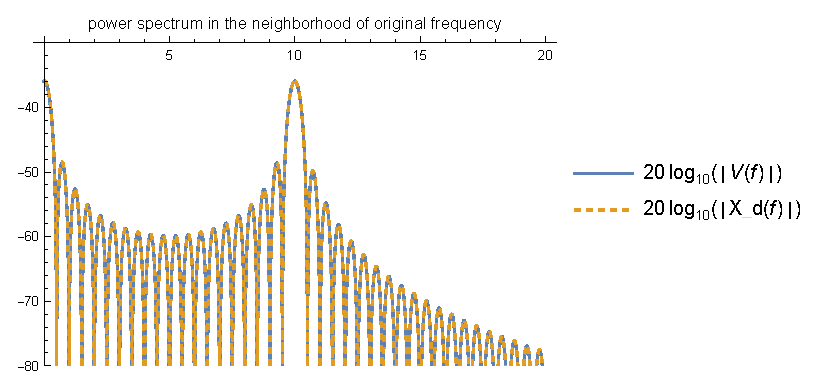
\includegraphics[keepaspectratio, scale=0.8]
                {\currfiledir/spectrum_in_the_neighborhood_of_original_frequency.eps}
                \caption{元の周波数の近傍でのパワースペクトル}
            \end{figure}
            低周波領域では絶対値が良く一致していることがわかる。
            \par
            次に高調波を見る。
            次の図はサンプリング周波数の3倍の範囲まで$V,\Xd$を示したものである。
            \begin{figure}[H]
                \centering
                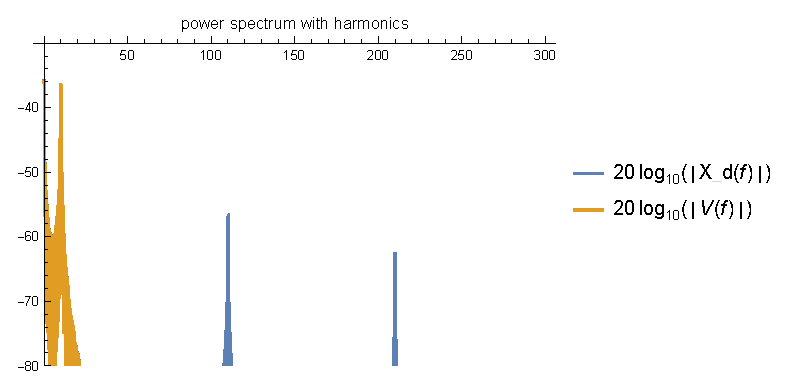
\includegraphics[keepaspectratio, scale=0.8]
                {\currfiledir/power_spectrum_with_harmonics.eps}
                \caption{高調波を含むパワースペクトル}
            \end{figure}
            低周波の領域では$V,\Xd$が重なって判別できない。
            また、サンプリング周波数の整数倍の位置に高調波が生じていることが判る。
            \par
            この数値例を計算したMathematicaノートブックおよびMATLABスクリプトは下記のファイル名で保存されている。
            Gitリポジトリ内でファイル名検索すれば発見できるであろう。
            \begin{itemize}
                \item \href{\currfiledir/spectrum_of_integral-sine-wave_by_Euler-method.nb}{spectrum\_of\_integral\-sine-wave\_by\_Euler-method.nb}
                \item \href{\currfiledir/spectrum_of_integral_sine_wave_by_Euler_method.m}{spectrum\_of\_integral\_sine\_wave\_by\_Euler\_method.m}
            \end{itemize}

